\documentclass[tikz,border=10pt]{standalone}
\usepackage{tikz}
\usetikzlibrary{calc, angles, quotes}

\begin{document}

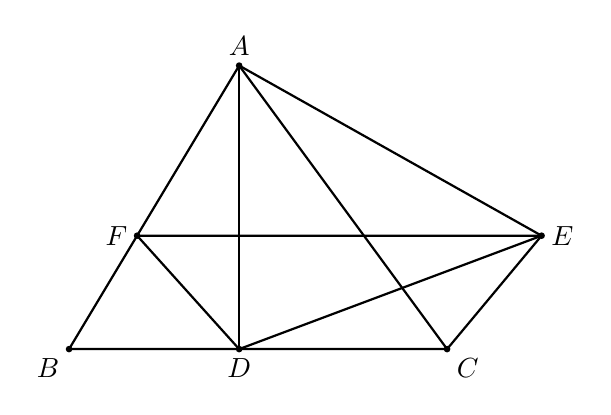
\begin{tikzpicture}[>=stealth, scale=1.2]
    % --- 1. 定义顶点坐标 (基于图像比例) ---
    \coordinate (B) at (0,0);
    \coordinate (C) at (4,0);
    \coordinate (A) at (1.8,3); % A点略微偏左

    % 计算 D 点 (BC 上的垂足或中点，此处根据原图表现为垂足附近)
    \coordinate (D) at (1.8,0); 

    % 计算 F 点 (AB 边上的点，约在靠下 1/3 处)
    \coordinate (F) at ($(A)!0.6!(B)$);

    % 计算 E 点 (位于右侧，使得 FE 呈水平或特定几何关系)
    \coordinate (E) at (5,1.2);

    % --- 2. 绘制主要实线段 ---
    \draw[thick] (B) -- (C) -- (A) -- cycle; % 绘制三角形 ABC
    \draw[thick] (A) -- (D);                 % 绘制高/中线 AD
    \draw[thick] (A) -- (E);                 % 绘制线段 AE
    \draw[thick] (F) -- (D);                 % 绘制线段 FD
    \draw[thick] (F) -- (E);                 % 绘制水平线 FE
    \draw[thick] (D) -- (E);                 % 绘制线段 DE
    \draw[thick] (C) -- (E);                 % 绘制线段 CE

    % --- 3. 绘制顶点标记 ---
    \node[above] at (A) {$A$};
    \node[below left] at (B) {$B$};
    \node[below] at (D) {$D$};
    \node[below right] at (C) {$C$};
    \node[left] at (F) {$F$};
    \node[right] at (E) {$E$};

    % --- 4. 绘制关键点圆点 (可选，增强学术感) ---
    \foreach \p in {A,B,C,D,E,F}
        \fill (\p) circle (1pt);

\end{tikzpicture}

\end{document}